% Section 1
% 2021-08-19
% Alessandro Zanatta

\section{Introduction}
\label{section:introduction}

Security protocols are used everyday by billions of users and applications to guarantee a certain degree of security and privacy over communications happening on the (insecure) Internet (MTProto2.0 \cite{Telegram-MTProto2.0}, Signal \cite{Signal} and TLSv1.3 \cite{TLSv1.3_specs} protocols are just a few famous examples). Although, there is a catch: designing such protocols has been proven to be very error prone. As an example, consider the Needham-Schroeder public-key protocol \cite{NSPK}, which has been considered secure for almost 20 years $-$ before a fatal flaw was found and corrected \cite{NSPK_LoweGavin}.

Given the importance of the correctness of such protocols and the difficulties for designers to ensure it, it has been necessary to \textit{formally} prove the absence of security vulnerabilities. Towards this aim, a set of tools have been developed to assist the designing process of a new protocol.

\subsection{Classification of tools}

\afterpage{
    \begin{figure}[t]
        \makebox[\textwidth][c]{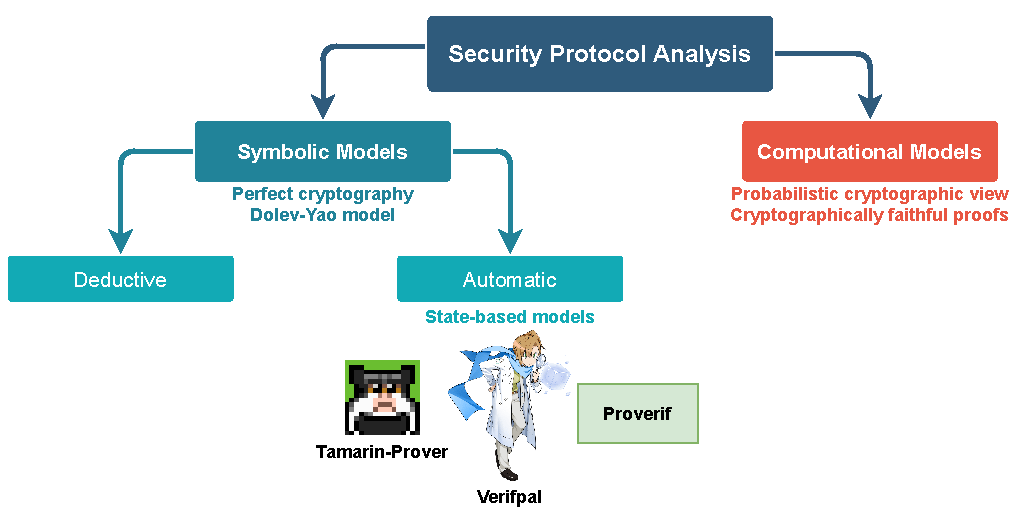
\includegraphics[scale=.9]{symbolic-computational-model}}
        \caption{Classification of tools}
        \label{fig:classification-of-tools}
    \end{figure}
}

These tools can be classified as shown in \cref{fig:classification-of-tools}. Two classes of tools can be identified. As the tools we are going to examine exploit the symbolic model, we will not explore the computational model (see \cite{ReconcilingComputationalSymbolic, SymbolicComputationalBlanchet, 10.1007/978-3-540-31987-0_12} for further readings). 

Let us briefly examine the symbolic model. This model assumes a Dolev-Yao \cite{Dolev-Yao} attacker. Moreover, cryptographic primitives are considered as black-box and are represented using function symbols, the messages are terms and the adversary can only use defined primitives. An important aspect to note of this model is that it assumes \textbf{perfect cryptography}. As an example, consider the case in which there are two function symbols (\textbf{enc} and \textbf{dec}, used to encrypt and decrypt), a message \textit{m} and a key \textit{k} and the following equality is defined:


\begin{equation}
\mbox{dec}\left(\mbox{enc}\left(m, k\right), k\right) = m
\end{equation}

Following from the equation $-$ and considering the perfect cryptography assumption $-$ it is possible to decrypt $\mbox{enc}\left(m, k\right)$ if and only if \textit{k} is known \cite{SymbolicComputationalBlanchet}.

We can further classify these tools in automatic and deductive. In particular, we will have a look at the internal reasoning and at some examples of three automatic tools: Tamarin-prover, Verifpal and Proverif.